\documentclass{beamer}

\usepackage{tikz, hyperref}
\usetikzlibrary{calc}

\author{Quang Tung Thai}
\title {Figures}


\begin{document}


\begin{frame}
  \frametitle{An example of network slicing}
  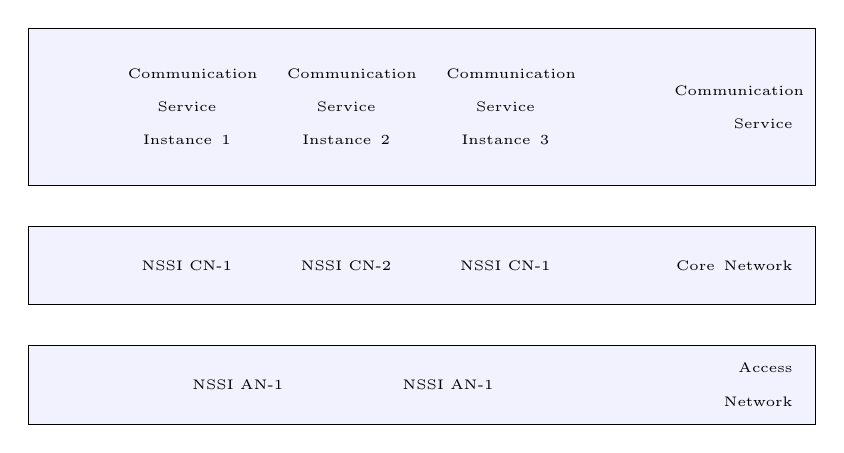
\begin{tikzpicture}[block/.style={rectangle,draw=black, minimum width=10cm, fill= blue!5}]
  
  \node[block, minimum height=1cm] at (0,0) (b1) {};
  \node[block, minimum height=1cm,above] at ([yshift=0.5cm]b1.north) (b2) {};
  \node[block, minimum height=2cm,above] at ([yshift=0.5cm]b2.north) (b3) {};
  \node[text width=1.5cm, left, align=right] at ([xshift=-5pt]b1.east) (l1) {\tiny Access Network};
  \node[text width=1.5cm, left, align=right] at ([xshift=-5pt]b2.east) (l2) {\tiny Core Network};
  \node[text width=1.5cm, left, align=right] at ([xshift=-5pt]b3.east) (l3) {\tiny Communication Service};  
  
  \node at ($(b1.west)!0.33!(l1.west)$) {\tiny NSSI AN-1};
  \node at ($(b1.west)!0.66!(l1.west)$) {\tiny NSSI AN-1};
  \node at ($(b2.west)!0.25!(l2.west)$) {\tiny NSSI CN-1};
  \node at ($(b2.west)!0.5!(l2.west)$) {\tiny NSSI CN-2};
  \node at ($(b2.west)!0.75!(l2.west)$) {\tiny NSSI CN-1};
  \node[text width=1.5cm, align=center] at ($(b3.west)!0.25!(l3.west)$) {\tiny Communication Service Instance 1};
  \node[text width=1.5cm, align=center] at ($(b3.west)!0.5!(l3.west)$) {\tiny Communication Service Instance 2};
  \node[text width=1.5cm, align=center] at ($(b3.west)!0.75!(l3.west)$) {\tiny Communication Service Instance 3};
      
  \end{tikzpicture}
\end{frame}

\end{document}